\documentclass{article}
\usepackage{cmap}
\usepackage[utf8]{inputenc}
\usepackage[english,ukrainian]{babel}
\usepackage{graphicx}
\usepackage{geometry}
\usepackage{listings}
\usepackage{float}
\geometry{
	a4paper,
	left=20mm,
	right=20mm,
	top=20mm,
	bottom=20mm
}
\lstset{
	language=c,
	tabsize=4,
	keepspaces,
	showstringspaces=false,
}
\graphicspath{ {./pictures} }
\setlength{\parindent}{4em}

\newcommand\subject{Алгоритми та структури даних}
\newcommand\lecturer{доцент кафедри ПЗ\\Коротєєва Т.О.}
\newcommand\teacher{асистент кафедри ПЗ\\Франко А.В.}
\newcommand\mygroup{ПЗ-22}
\newcommand\lab{1}
\newcommand\theme{Метод сортування бульбашкою}
\newcommand\purpose{Вивчити алгоритм сортування бульбашкою. Здійснити програмну реалізацію алгоритму сортування бульбашкою. Дослідити швидкодію алгоритму сортування бульбашкою}

\begin{document}
\begin{normalsize}
	\begin{titlepage}
		\thispagestyle{empty}
		\begin{center}
			\textbf{МІНІСТЕРСТВО ОСВІТИ І НАУКИ УКРАЇНИ\\
				НАЦІОНАЛЬНИЙ УНІВЕРСИТЕТ "ЛЬВІВСЬКА ПОЛІТЕХНІКА"}
		\end{center}
		\begin{flushright}
			Інститут \textbf{КНІТ}\\
			Кафедра \textbf{ПЗ}
		\end{flushright}
		\vspace{200pt}
		\begin{center}
			\textbf{ЗВІТ}\\
			\vspace{10pt}
			До лабораторної роботи № \lab\\
			\textbf{На тему}: “\textit{\theme}”\\
			\textbf{З дисципліни}: “\subject”
		\end{center}
		\vspace{112pt}
		\begin{flushright}
			
			\textbf{Лектор}:\\
			\lecturer\\
			\vspace{28pt}
			\textbf{Виконав}:\\
			
			студент групи \mygroup\\
			Коваленко Д.М.\\
			\vspace{28pt}
			\textbf{Прийняв}:\\
			
			\teacher\\
			
			\vspace{28pt}
			«\rule{1cm}{0.15mm}» \rule{1.5cm}{0.15mm} 2022 р.\\
			$\sum$ = \rule{1cm}{0.15mm}……………\\
			
		\end{flushright}
		\vspace{\fill}
		\begin{center}
			\textbf{Львів — 2022}
		\end{center}
	\end{titlepage}
		
	\begin{description}
		\item[Тема.] \theme.
		\item[Мета.] \purpose.
	\end{description}

	\section*{Лабораторне завдання}
	Створити віконний проект та написати програму, яка реалізує алгоритм сортування бульбашкою.
	\begin{center}
		2. Задано перелік товарів у супермаркеті та їх ціни. Упорядкувати за алфавітом лише ті товари, вартість яких не перевищує середню.
	\end{center}
	
	\section*{Теоретичні відомості}
	Загальна задача сортування полягає в наступному: нехай дано множину елементів, яка є індексованою, тобто довільно пронумерованою від $1$ до $n$. Необхідно індексувати цю множину елементів так, щоб з умови $i<j$ витікало $a_i < а_j$ - для всіх $i,j=1..n$. Отже, процес сортування полягає у послідовних перестановках елементів доти, доки їх індексація не узгодиться з їх впорядкованістю.
	
	Алгоритм сортування бульбашкою (англійською «Bubble Sort») відноситься до класу алгоритмів сортування вибіркою. Алгоритм працює наступним чином — у заданому наборі даних (списку чи масиві) порівнюються два сусідні елементи. Якщо один з елементів не відповідає критерію сортування (є більшим, або ж, навпаки, меншим за свого сусіда), то ці два елементи обмінюються місцями. Прохід по масиву продовжується до тих пір, доки дані не будуть відсортованими. 
	Алгоритм отримав свою назву від того, що процес сортування згідно нього нагадує поведінку бульбашок повітря у резервуарі з водою: найлегша бульбашка піднімається до гори першою. Оскільки для роботи з елементами масиву алгоритм використовує лише порівняння, це сортування на основі порівнянь.
	
	Цей метод неефективний для масивів великого розміру. Існує багато модифікацій даного алгоритму.
	
	\subsection*{Покроковий опис роботи алгоритму сортування бульбашкою}
	\textbf{Алгоритм В}
	Задано масив елементів $R_1$ ,$R_2$ ,…,$R_n$. F – прапорець перестановок.\\
	Даний алгоритм реорганізує масив у висхідному порядку, тобто для його елементів буде мати місце співвідношення $R_i < R_j$ - для всіх $i,j=1..n$.\\
	В1. Цикл за індексом проходження. Повторювати кроки В2 і В3 при $i=1..n-1$.\\
	В2. Ініціалізація прапорця перестановки: встановити $F=0$.\\
	В3. Виконання проходження. Повторювати при $j=1,2,…,n-i$ : якщо $R_{j+1} < R_j$ , то встановити F=1 та переставити місцями елементи $R_j$<->$R_j+1$, ; якщо $F=0$, то завершити виконання алгоритму. \\
	В4. Кінець. Вихід.
	
	\section*{Хід роботи}
	\subsection*{Файл sort.rs}
	\begin{lstlisting}
use crate::data::Data;

pub struct Sorted;

impl Sorted {
	pub fn sort(v: &mut Vec<Data>) -> Vec<(usize, usize)> {
		remove_above_avg_price(v);
		let mut sorted = false;
		let mut res = Vec::new();
		for i in 0..v.len() {
			for j in 0..(v.len() - 1 - i) {
				sorted = true;
				if v[j] > v[j + 1] {
					v.swap(j, j + 1);
					res.push((j, j + 1));
					sorted = false;
				}
			}
			if sorted { break }
		}
		res
	}
}

fn remove_above_avg_price(v: &mut Vec<Data>) {
	let avg_price = v.iter().map(|d| d.price).sum::<f32>() / v.len() as f32;
	v.retain(|d| d.price < avg_price);
}\end{lstlisting}
	\subsection*{Файл data.rs}
	\begin{lstlisting}
use fake::{faker::lorem::en::*, Dummy, Fake};

#[derive(Debug, Clone, PartialEq, Dummy)]
pub struct Data {
	#[dummy(faker = "Word()")]
	pub name: String,
	pub price: f32,
}

impl PartialOrd for Data {
	fn partial_cmp(&self, other: &Self) -> Option<std::cmp::Ordering> {
		self.name.partial_cmp(&other.name)
	}
}\end{lstlisting}
	\subsection*{Файл main.rs}
	\begin{lstlisting}
mod data;
mod sort;

use eframe::egui;
use egui_extras::{Size, TableBuilder};

use crate::{data::Data, sort::Sorted};

fn main() {
	let options = eframe::NativeOptions::default();
	eframe::run_native(
	"Sorting",
	options,
	Box::new(|_cc| Box::new(SortingApp::new())),
	);
}

struct SortingApp {
	data: Option<Vec<Data>>,
	prev_data: Option<Vec<Data>>,
	data_len: usize,
	selected: Option<Vec<(usize, usize)>>,
	elapsed: Option<std::time::Duration>,
}

impl SortingApp {
	fn new() -> Self {
		Self {
			data: Some(fake::vec![Data; 1]),
			prev_data: None,
			data_len: 1,
			selected: None,
			elapsed: None,
		}
	}
}

impl eframe::App for SortingApp {
	fn update(&mut self, ctx: &egui::Context, _frame: &mut eframe::Frame) {
		egui::CentralPanel::default().show(ctx, |ui| {
			if ui
			.add(egui::DragValue::new(&mut self.data_len).speed(0.1))
			.changed
			{
				self.data = Some(fake::vec![Data; self.data_len])
			}
			ui.end_row();
			if ui.button("Sort").clicked() {
				self.prev_data = self.data.to_owned();
				match &mut self.data {
					Some(d) => {
						use std::time::Instant;
						let now = Instant::now();
						self.selected = Some(Sorted::sort(d));
						self.data_len = d.len();
						self.elapsed = Some(now.elapsed());
					}
					None => {}
				};
			}
			if let Some(elapsed) = self.elapsed {
				ui.label(format!("{:.2?}", elapsed).to_string());
			}
			ui.end_row();
			egui::Grid::new("unique_id")
			.min_col_width(290.)
			.show(ui, |ui| {
				ui.label("after");
				ui.label("before");
				ui.label("Indexes");
				ui.end_row();
			});
			egui::Grid::new("another_unique_id")
			.min_row_height(500.)
			.show(ui, |ui| {
				ui.push_id(1, |ui| {
					TableBuilder::new(ui)
					.striped(true)
					.cell_layout(egui::Layout::left_to_right(egui::Align::Center))
					.column(Size::initial(20.0).at_least(40.0))
					.column(Size::initial(150.0).at_least(40.0))
					.column(Size::initial(100.0).at_least(40.0))
					.body(|mut body| {
						if let Some(data) = self.data.as_ref() {
							for i in 0..data.len() {
								body.row(30., |mut row| {
									row.col(|ui| {
										ui.label(i.to_string());
									});
									row.col(|ui| {
										if let Some(v) = data.get(i) {
											ui.label(v.name.clone());
										}
									});
									row.col(|ui| {
										if let Some(v) = data.get(i) {
											ui.label(v.price.to_string());
										}
									});
								});
							}
						}
					});
				});
				
				ui.push_id(2, |ui| {
					TableBuilder::new(ui)
					.striped(true)
					.cell_layout(egui::Layout::left_to_right(egui::Align::Center))
					.column(Size::initial(20.0).at_least(40.0))
					.column(Size::initial(150.0).at_least(40.0))
					.column(Size::initial(100.0).at_least(40.0))
					.body(|mut body| {
						if let Some(data) = self.prev_data.as_ref() {
							for i in 0..data.len() {
								body.row(30., |mut row| {
									row.col(|ui| {
										ui.label(i.to_string());
									});
									row.col(|ui| {
										if let Some(v) = data.get(i) {
											ui.label(v.name.clone());
										}
									});
									row.col(|ui| {
										if let Some(v) = data.get(i) {
											ui.label(v.price.to_string());
										}
									});
								});
							}
						}
					});
				});
				
				ui.push_id(3, |ui| {
					TableBuilder::new(ui)
					.striped(true)
					.cell_layout(egui::Layout::left_to_right(egui::Align::Center))
					.column(Size::initial(40.0).at_least(40.0))
					.column(Size::initial(40.0).at_least(40.0))
					.body(|mut body| {
						if let Some(selected) = self.selected.as_ref() {
							for i in 0..selected.len() {
								body.row(30., |mut row| {
									row.col(|ui| {
										if let Some(v) = selected.get(i) {
											ui.label(v.0.to_string());
										}
									});
									row.col(|ui| {
										if let Some(v) = selected.get(i) {
											ui.label(v.1.to_string());
										}
									});
								});
							}
						}
					});
				});
			});
		});
	}
}\end{lstlisting}

	\begin{figure}[H]
		\centering
		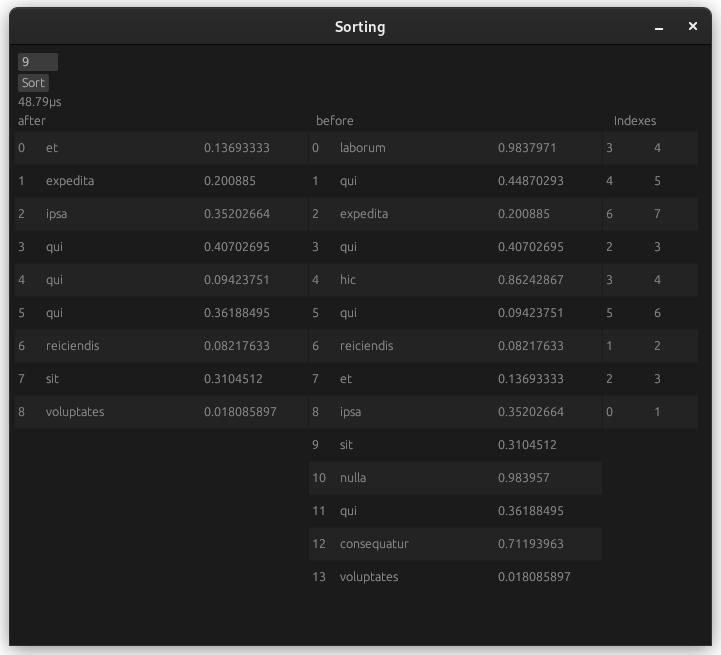
\includegraphics[scale=0.7]{1}
		\caption{Виконання програми}
	\end{figure}
	
	\section*{Висновок}
	Під час виконання лабораторної роботи я навчився використовувати алгоритм сортування бульбашкою. Програмно реалізував алгоритм та дослідив його швидкодію.
	    
\end{normalsize}
\end{document}
